% xcolor=table is because it seems that beamer uses the xcolor package in a
% strange way and thus don't accept us giving arguments to the package.
\documentclass[slidestop,compress,mathserif, xcolor=table]{beamer}

\usepackage[T1]{fontenc}
\usepackage[utf8]{inputenc}
\usepackage[english]{babel}
\usepackage{listings}

\lstset{
    language=c,                        % choose the language of the code
    basicstyle=\ttfamily\footnotesize, % the size of the fonts that are used for the
    keywordstyle=,
    numbers=left,                      % where to put the line-numbers
    numberstyle=\footnotesize,         % the size of the fonts that are used for the
    numbersep=5pt,                     % how far the line-numbers are from the code
    backgroundcolor=\color{white},     % choose the background color. You must add
    showspaces=false,                  % show spaces adding particular underscores
    showstringspaces=false,            % underline spaces within strings
    showtabs=false,                    % show tabs within strings adding particular
    frame=single,                      % adds a frame around the code
    breaklines=true,                   % sets automatic line breaking
    breakatwhitespace=false            % sets if automatic breaks should only happen at
}

% \usepackage{mdwtab}
% \usepackage{mathenv}
% \usepackage{amsfonts}
% \usepackage{amsmath}
% \usepackage{amssymb}
% \usepackage{amsthm}

\usepackage{semantic}
\renewcommand{\ttdefault}{txtt} % Bedre typewriter font

% Use the NAT theme in uk (also possible in DK)
\usetheme[nat,uk, footstyle=low, TPrawlrimage=pony.jpg]{Frederiksberg}

\definecolor{mypink}{RGB}{255,200,220}
\setbeamercolor{background canvas}{bg=mypink}
%\setbeamercolor{structure}{fg=blue}

% Make overlay sweet nice by having different transparancy depending on how
% "far" ahead the overlay is. AWSOME!!
%\setbeamercovered{highly dynamic}
% possible to shift back, so they are just invisible untill they should overlay
% \setbeamercovered{invisible}

% Extend figures into either left or right margin
% Ex: \begin{narrow}{-1in}{0in} .. \end{narrow} will place 1in into left margin
\newenvironment{narrow}[2]{%
  \begin{list}{}{%
  \setlength{\topsep}{0pt}%
  \setlength{\leftmargin}{#1}%
  \setlength{\rightmargin}{#2}%
  \setlength{\listparindent}{\parindent}%
  \setlength{\itemindent}{\parindent}%
  \setlength{\parsep}{\parskip}}%
\item[]}{\end{list}}



\usepackage{tikz}
\usetikzlibrary{calc,shapes,arrows}
% below is for use of backgrounds (foregrounds are not used so they are not
% added to this specification).
\pgfdeclarelayer{background}
\pgfsetlayers{background,main}


\usepackage{subfigure}


% Write a short text to have that shown in the footer of slides other than the
% title slide.
\title[]{Lær at lave stack pwnyflows}
% A possible subslide.
%\subtitle{Regular-expression based bit coding}


\author[br0ns \and iDolf Hatler \and TM]
       {br0ns \and iDolf Hatler \and TM}

% Only write DIKU in the footer of slides (except the title slide).
\institute[DIKU]{Datalogisk institut, Københavns universitet}

% Remove the date stamp from the footer of slides (except title slide) by giving
% it no short "text"
\date[]{\today}

\begin{document}

\frame[plain]{\titlepage}

\begin{frame}[c]
    \frametitle{Aftenens Program}

    \begin{itemize}
        \pause\item Lær at bruge gdb
        \pause\item Lær at læse gcc-genereret assembler
        \pause\item Lær at bruge jeres tidligere udviklede shellcode
    \end{itemize}
\end{frame}

\begin{frame}[c]
    \frametitle{Stakken og funktionskald}
    \begin{itemize}
        \pause\item Frames og funktioner
        \pause\item Argumenter
        \pause\item Returadresse, gemt basepointer
        \pause\item Variable
    \end{itemize}
\end{frame}

\begin{frame}[c]
    \frametitle{Stakken med frames, visuelt}
    \begin{center}
        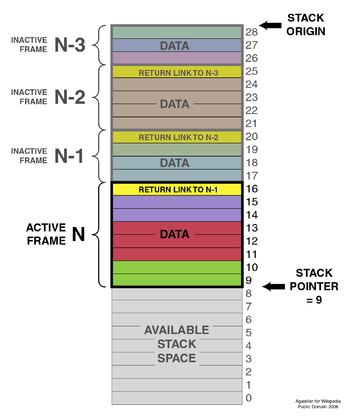
\includegraphics[height=.75\textheight]{ProgramCallStack2}
    \end{center}
\end{frame}

\begin{frame}[c]
    \frametitle{Konkret eksempel}

    \pause\lstinputlisting{foo.c}

    \pause\lstinputlisting{foo.asm}

\end{frame}

\begin{frame}[c]
    \frametitle{Oversigt over stakken}

    Dette er sådan stakken (normalt) ser ud. $a$ er antallet af (4-bytes)
    argumenter, $v$ er antallet af (4-bytes) lokale variable. \vskip8pt

    \pause\emph{OBS:} $v$ er ikke det egentlig antal lokale variable, idet GCC
    laver padding og arrays typisk fylder mere end 4 bytes. \vskip8pt

    \pause
    \begin{tabular}{|l|l|c|}
    \hline
    \texttt{[ebp+0x8$+4n$]} & \texttt{[esp$+4v$+0x8$+4n$]}  & Argument nummer $n$ \\
                            &                               & (hvor $0 \leq n < a$) \\\hline
    \texttt{[ebp+0x4]}      & \texttt{[esp$+4v$+0x4]}       & Returadressen \\\hline
    \texttt{[ebp]}          & \texttt{[esp$+4v$]}           & Den gamle værdi af \texttt{ebp}\\\hline
    \texttt{[ebp$-4v+4n$]}  & \texttt{[esp$+4n$]}           & Lokal variabel position \\
                            &                               & $n$ (hvor $0 \leq n < v$) \\\hline
    \end{tabular}
\end{frame}

\begin{frame}[c]
    \frametitle{Fornuftige gdb-indstillinger}

    \texttt{$\sim$/.gdbinit} (\texttt{mv dotgdbinit $\sim$/.gdbinit})

    \lstinputlisting{gdbinit}

    Start typisk med:
    \lstinputlisting{gdbintro}
\end{frame}

\begin{frame}[c,volatile]
    \frametitle{Basal GDB}

    \begin{center}
    \begin{tabular}{|l|c|}
    \hline
    \texttt{disas [funktion]} & Disassembler en funktion \\\hline
    \texttt{b [funktion]}     & Sæt et breakpoint \\\hline
    \texttt{c}                & Fortsæt indtil næste breakpoint \\\hline
    \texttt{run}              & Starter kørslen \\\hline
    \texttt{x [arg]}          & \texttt{help x}, eks. \texttt{x/20i \$esp}\\
                              & Giver 20 instruktioner fra esp\\\hline
    \texttt{disp}             & Som \texttt{x}, men gentages efter hvert step
    \\\hline

    \texttt{i r}              & Giver informationer om alle registre\\\hline
    \texttt{si}               & Træder en instruktion frem\\\hline
    \texttt{ni}               & Som \texttt{si}, men følger ikke
    funktionskald\\\hline
    \end{tabular}
    \end{center}

    Start typisk med:
    \lstinputlisting{gdbintro}
\end{frame}

\begin{frame}[c]
    \frametitle{Legetime1}

    \pause
    {\footnotesize
      Legetime 1: 
        Disasemble legetime1:
        \begin{itemize}
            \item Undersøg hvor mange argumenter programmet tager
            \item Find og print argumenterne til main
            \item Hvilke argumenter bliver givet til de forskellige funktioner
            \item Hvad gør de forskellige funktioner.\\
            Hint: man printf
            \item Hvad gør programmet
        \end{itemize}
\end{frame}

\begin{frame}[c]
    \frametitle{Stackoverflow}
    \pause
    \lstinputlisting{foo2.c}
\end{frame}


\begin{frame}[c]

      \item Legetime 2: Find et stack overflow i funktionen \texttt{log\_string}
        og udnyt det. Det vil være en klar fordel at læse og forstå hvad
        funktionen gør. Der findes en smart funktion som du gerne vil overskrive
        returadressen med - du finder den funktion ved at køre kommandoen
        \texttt{readelf -s legetime2 | grep FUNC}.

      \item Legetime 3: \texttt{legetime4} er næsten identisk med
        \texttt{legetime2}. Den smarte funktion fra før er fjernet, til gengæld
        får du mulighed for at finde din shellcode frem.

      \item Ekstraopgaver: Løs så mange baner af IO på Smash the stack som
        du kan: \url{http://io.smashthestack.org}.

      % \item Legetime 5: Du har nu ikke længere mulighed for at køre shellcode på
      %   en kendt adresse - hvad gør du så? Hint: \texttt{zero\_buffers} kan
      %   \emph{ikke} exploites, men er der alligevel af en årsag.

      \end{itemize}
    }
\end{frame}

\end{document}
